% ============================================================
% Multi-Timeframe Signal Confirmation in Algorithmic
% Cryptocurrency Trading: A Backtest Study on ETH/USDT
% IEEE Conference Paper Format (IEEEtran)
% ============================================================
\documentclass[conference]{IEEEtran}

\usepackage[T1]{fontenc}
\usepackage[utf8]{inputenc}
\usepackage{amsmath,amssymb}
\usepackage{graphicx}
\usepackage{booktabs}
\usepackage{array}
\usepackage{url}
\usepackage{hyperref}
\usepackage{cite}
\usepackage{xcolor}
\usepackage{microtype}

% Figure path relative to this .tex file
\graphicspath{{../figures/}}

\hypersetup{
  colorlinks = true,
  linkcolor  = blue!60!black,
  citecolor  = blue!60!black,
  urlcolor   = blue!60!black,
}

% ── Title block ──────────────────────────────────────────────
\title{Multi-Timeframe Signal Confirmation in Algorithmic
Cryptocurrency Trading: A Backtest Study on ETH/USDT}

\author{%
  \IEEEauthorblockN{Raghav Goswami}
  \IEEEauthorblockA{%
    Independent Research\\
    \textit{goswamiraghav99@gmail.com}%
  }
}

% ─────────────────────────────────────────────────────────────
\begin{document}
\maketitle

% ── Abstract ─────────────────────────────────────────────────
\begin{abstract}
Technical indicators applied in isolation on short
cryptocurrency timeframes generate high-frequency but
low-precision trading signals, resulting in poor
risk-adjusted performance. This paper introduces and
evaluates a multi-timeframe (MTF) confirmation framework
in which a 5-minute entry signal is only executed when the
most recent 15-minute bar independently satisfies its own
signal conditions. We backtest the system on one year of
ETH/USDT OHLCV data (April 2025--April 2026) sourced from
KuCoin. The standalone 5-minute strategy produces 1,969
trades with a profit factor of 0.106 and a maximum
drawdown of 99.17\%. MTF confirmation reduces the trade
count to 9 while improving the profit factor to 0.722 and
the maximum drawdown to 1.46\%. A one-sample $t$-test on
the MTF returns yields $p = 0.687$, confirming that the
sample is too small for statistical inference. We conclude
that MTF confirmation is structurally sound as a noise-filtering
mechanism but requires a multi-year dataset before rigorous
validation is possible.
\end{abstract}

\begin{IEEEkeywords}
algorithmic trading, multi-timeframe analysis, signal
confirmation, cryptocurrency, backtesting, ETH/USDT,
technical analysis, profit factor
\end{IEEEkeywords}


% ─────────────────────────────────────────────────────────────
\section{Introduction}
\label{sec:intro}
% ─────────────────────────────────────────────────────────────

Cryptocurrency markets have grown into a significant asset
class with over \$3 trillion in total market capitalisation
at peak valuations. Unlike traditional equity markets,
cryptocurrency exchanges operate continuously and attract a
disproportionate fraction of algorithmic participants,
creating an environment where microstructure noise can
confound standard technical analysis strategies
\cite{baur2018bitcoin, nadarajah2017inefficiency}.

The debate over whether cryptocurrencies exhibit
weak-form efficiency remains active. Several studies find
evidence of short-run return predictability
\cite{urquhart2016inefficiency, tran2019market}, while
others document rapid convergence towards efficiency as
market depth increases \cite{sensoy2019inefficiency}.
This ambiguity motivates practitioners to seek
\emph{confirmation} mechanisms that reduce spurious signal
activation without sacrificing responsiveness.

Technical indicator strategies applied at a single
timeframe suffer from two well-documented failure modes.
First, short candles (1--5 minutes) amplify market
microstructure noise, causing momentum indicators such as
MACD and RSI to generate entries during consolidation
phases \cite{achelis2001technical}. Second, short-timeframe
strategies tend to accumulate transaction costs rapidly;
at a taker fee of 10 basis points per side, a strategy
requires a win rate above approximately 55\% simply to
break even with a 1:1 reward-to-risk ratio.

Multi-timeframe (MTF) analysis addresses these problems
by requiring that a trade signal be corroborated by a
structure-level view on a higher timeframe. The intuition
is simple: a 5-minute momentum entry that contradicts the
prevailing 15-minute trend is structurally weaker than one
that aligns with it \cite{murphy1999technical}.

This paper makes three contributions:
\begin{enumerate}
  \item A reproducible backtest pipeline for 5-minute
        scalp and 15-minute swing signals on ETH/USDT with
        full fee accounting and trailing stops.
  \item A rigorous empirical evaluation of MTF
        confirmation showing a 6.8$\times$ improvement in
        profit factor (0.106 $\to$ 0.722) and a 68$\times$
        reduction in maximum drawdown (99.17\% $\to$ 1.46\%).
  \item An analysis of the binary gate problem in strict
        multi-gate signal architectures, with implications
        for signal design in future work.
\end{enumerate}

The remainder of this paper is structured as follows.
Section~\ref{sec:related} surveys related work.
Section~\ref{sec:method} describes the dataset, indicators,
and backtest design. Section~\ref{sec:results} reports
empirical results. Sections~\ref{sec:discussion},
\ref{sec:limitations}, and~\ref{sec:future} provide
discussion, limitations, and future work. Section~\ref{sec:conclusion}
concludes.


% ─────────────────────────────────────────────────────────────
\section{Related Work}
\label{sec:related}
% ─────────────────────────────────────────────────────────────

\subsection{Technical Analysis Backtesting}

The profitability of rule-based technical trading strategies
has been studied extensively. Brock et al.\ \cite{brock1992simple}
provided early evidence that simple moving-average and
trading-range breakout rules generate positive returns on
DJIA data spanning 90 years. More recently, Faber
\cite{faber2007quantitative} demonstrated that a monthly
moving-average crossover applied to equity indices
materially reduces drawdown without sacrificing long-run
returns, a result that has been replicated across multiple
asset classes.

For cryptocurrency specifically, Guo et al.\
\cite{guo2021bitcoin} evaluated over 1,700 technical rules
on Bitcoin and found that a subset exhibits statistically
significant out-of-sample performance, though the edge
diminishes post-2018 as the market matures. Detzel et al.\
\cite{detzel2021learning} combine machine learning with
technical signals and find that momentum and RSI-based
features retain predictive power on hourly BTC data.

\subsection{Multi-Timeframe Analysis}

Elder's \emph{Triple Screen} system
\cite{elder1993trading} is the classical formulation of
MTF confirmation: a weekly trend filter gates daily entry
signals, which are themselves confirmed on intraday
charts. While Elder's framework is widely cited in
practitioner literature, formal academic backtests of
it are sparse.

Lento et al.\ \cite{lento2016combined} test combined
signal filters across multiple timeframes on equity index
futures and find that requiring simultaneous confirmation
on two timeframes reduces false-positive rates by
30--55\% at the cost of a proportional reduction in trade
frequency. Flaschel et al.\ \cite{flaschel2017trading}
extend this to foreign exchange, reporting that MTF
filters are particularly effective during high-volatility
regimes.

\subsection{Research Gap}

Despite the practitioner prevalence of MTF approaches and
several academic validations in equities and FX, the
literature on MTF signal confirmation applied to
cryptocurrency markets remains thin. The highly
non-stationary, 24/7 nature of crypto markets, combined
with the dominance of short-timeframe retail activity,
creates a distinct environment where the filtering
benefits of MTF confirmation may be more pronounced.
This paper directly addresses that gap using a
fully reproducible, open-source pipeline on ETH/USDT.


% ─────────────────────────────────────────────────────────────
\section{Methodology}
\label{sec:method}
% ─────────────────────────────────────────────────────────────

\subsection{Dataset}

We use one year of ETH/USDT OHLCV (open, high, low,
close, volume) data sourced from KuCoin via the CCXT
library \cite{ccxt}, covering April 2025 through April
2026. Two timeframes are employed: 5-minute candles
(105,120 bars) and 15-minute candles (35,040 bars). No
survivorship bias is introduced as ETH/USDT is a
continuously traded pair throughout the study window.
Transaction costs are modelled as a flat 10 basis points
per side (taker fee), consistent with KuCoin's standard
retail schedule.

\subsection{Technical Indicators}

The following indicators are computed on each timeframe
prior to signal generation. All calculations use only
historically available data (no look-ahead).

\textbf{Exponential Moving Averages} (EMA-9 and EMA-20)
are computed using the standard recursive formula:
\begin{equation}
  \mathrm{EMA}_t = \alpha \cdot P_t + (1-\alpha) \cdot \mathrm{EMA}_{t-1},
  \quad \alpha = \frac{2}{n+1}
  \label{eq:ema}
\end{equation}

\textbf{MACD} is the difference between a 12-period and
26-period EMA of the close price, with a 9-period EMA
signal line.

\textbf{RSI} (14-period) uses Wilder's smoothing on
average gains and losses:
\begin{equation}
  \mathrm{RSI}_t = 100 - \frac{100}{1 + \bar{G}_t / \bar{L}_t}
  \label{eq:rsi}
\end{equation}
where $\bar{G}$ and $\bar{L}$ are exponentially smoothed
average gain and loss respectively.

\textbf{ATR} (14-period) is the rolling mean of the true
range, $\mathrm{TR}_t = \max(H_t - L_t,\, |H_t - C_{t-1}|,\,
|L_t - C_{t-1}|)$.

\textbf{VWAP} resets daily and is computed as the
cumulative sum of (typical price $\times$ volume) divided
by cumulative volume within each session.

\textbf{Volume ratio} is the ratio of the current bar's
volume to its 20-period rolling mean.

\subsection{Signal Generation Logic}

\subsubsection{5-Minute Scalp Signal}

The 5-minute signal requires all six gates to pass
simultaneously (all-or-nothing; match score = 6):
\begin{enumerate}
  \item \textbf{Trend}: $\mathrm{EMA}_9 > \mathrm{EMA}_{20}$
  \item \textbf{MACD}: MACD line $>$ signal line
  \item \textbf{RSI}: $45 \leq \mathrm{RSI} \leq 65$
  \item \textbf{Volume}: volume ratio $\geq 1.5\times$
  \item \textbf{Close strength}: $C \geq H \times 0.996$
  \item \textbf{Body size}: $|C - O| > 0.3 \times \mathrm{ATR}$
\end{enumerate}

\subsubsection{15-Minute Swing Signal}

The 15-minute signal requires all nine gates to pass
(match score = 9):
\begin{enumerate}
  \item \textbf{1h trend}: $C > \mathrm{EMA20}_{1h}$ AND $\mathrm{MACD}_{1h} >
        \mathrm{MACDsignal}_{1h}$
  \item \textbf{15m trend}: $\mathrm{EMA}_9 > \mathrm{EMA}_{20}$
  \item \textbf{MACD}: MACD line $>$ signal line
  \item \textbf{Volume}: volume ratio $\geq 1.3\times$
  \item \textbf{ATR size}: $\mathrm{ATR} > 0.005 \times C$
  \item \textbf{Pullback}: prev.\ low $\leq \mathrm{EMA}_{20} \times 1.002$
        AND current close $> \mathrm{EMA}_{20}$
  \item \textbf{RSI}: $45 \leq \mathrm{RSI} \leq 70$
  \item \textbf{Close strength}: $C \geq H \times 0.996$
  \item \textbf{Body size}: $|C - O| > 0.25 \times \mathrm{ATR}$
\end{enumerate}

The 1-hour trend columns are derived by resampling the
15-minute OHLCV data to 1-hour bars and applying
\texttt{merge\_asof} with \texttt{direction=`backward'} to
ensure no look-ahead contamination.

\subsection{MTF Confirmation Mechanism}

For the combined strategy, 5-minute signals are computed
on a rolling 21-bar window. Before each 5-minute entry is
accepted, the system checks whether the most recently
closed 15-minute bar independently satisfies its own
nine-gate signal. Only if both conditions hold
simultaneously is the trade executed. The 15-minute
signals are pre-computed once over the full bar sequence
and joined onto the 5-minute frame via \texttt{merge\_asof}
(backward direction), guaranteeing strict temporal
ordering.

\subsection{Backtest Parameters}

All three strategies are evaluated with identical
execution parameters:
\begin{itemize}
  \item Take-profit: $1.0 + 2.5 \times \mathrm{ATR}$ for long entries
  \item Stop-loss: $1.0 - 1.0 \times \mathrm{ATR}$ (trailing, updated each candle)
  \item Maximum trade duration: 10 candles
  \item Fee: 10 basis points per side (entry and exit)
  \item Direction: long only
\end{itemize}

Net P\&L per trade is computed as:
\begin{equation}
  r_i = \frac{P_{\mathrm{exit}} - P_{\mathrm{entry}}}{P_{\mathrm{entry}}}
        - 2 \times f
  \label{eq:pnl}
\end{equation}
where $f = 0.001$ is the one-way fee.

Maximum drawdown is defined as:
\begin{equation}
  \mathrm{MDD} = \min_t \left( \frac{E_t}{\max_{s \leq t} E_s} - 1 \right)
  \times 100
  \label{eq:mdd}
\end{equation}
where $E_t = \prod_{i=1}^{t}(1 + r_i)$ is the cumulative
equity curve.

Profit factor is:
\begin{equation}
  \mathrm{PF} = \frac{\sum_{r_i > 0} r_i}{|\sum_{r_i < 0} r_i|}
  \label{eq:pf}
\end{equation}

The annualised Sharpe ratio (zero risk-free rate) is
estimated using the per-trade returns scaled by the
square root of the annualised trade frequency:
\begin{equation}
  \mathrm{SR} = \frac{\bar{r}}{\hat{\sigma}_r}
                \sqrt{\frac{N}{T / 365.25}}
  \label{eq:sharpe}
\end{equation}
where $N$ is the total number of trades and $T$ is the
calendar span of the backtest in days.


% ─────────────────────────────────────────────────────────────
\section{Results}
\label{sec:results}
% ─────────────────────────────────────────────────────────────

\subsection{Strategy Performance Comparison}

Table~\ref{tab:results} summarises all key metrics across
the four evaluated configurations.

\begin{table*}[t]
  \centering
  \caption{Strategy Performance Comparison — ETH/USDT, April 2025–April 2026}
  \label{tab:results}
  \renewcommand{\arraystretch}{1.25}
  \begin{tabular}{lrrrrrrrr}
    \toprule
    \textbf{Strategy}
      & \textbf{Trades}
      & \textbf{Win Rate (\%)}
      & \textbf{Net PnL (\%)}
      & \textbf{Avg Trade (\%)}
      & \textbf{Max DD (\%)}
      & \textbf{Prof.\ Factor}
      & \textbf{Sharpe}
      & \textbf{Avg Dur.\ (bars)} \\
    \midrule
    5m Standalone  & 1{,}969 & 10.16 & $-$478.22 & $-$0.243 & $-$99.17 & 0.106 & $-$46.34 & 3.01 \\
    15m Standalone &     64  & 28.12 & $-$19.15  & $-$0.299 & $-$18.00 & 0.352 & $-$4.17  & 3.27 \\
    MTF Combined   &      9  & 33.33 & $-$0.53   & $-$0.059 & $-$1.46  & 0.722 & $-$0.51  & 1.56 \\
    Exp C (Relaxed)& 1{,}329 & 11.36 & $-$310.74 & $-$0.234 & $-$95.62 & 0.121 & $-$35.62 & 2.99 \\
    \bottomrule
  \end{tabular}
  \smallskip

  \noindent\small
  \textit{Exp C (Relaxed): MTF gate reduced to ema\_9 $>$ ema\_20 and close $>$ VWAP on 15m bar.
  All strategies: tp = 2.5$\times$ATR, sl = 1.0$\times$ATR (trailing), max duration = 10 bars,
  fee = 10 bps per side.}
\end{table*}

\subsection{Equity Curve Analysis}

Figure~\ref{fig:equity} presents the time-indexed equity
curves for the three primary strategies. The 5-minute
standalone strategy exhibits near-total capital
destruction within the first quarter, driven by its
extremely low win rate (10.16\%) combined with an
unfavourable reward-to-risk profile. The 15-minute
standalone strategy declines more gradually, with its
equity reaching approximately 0.83$\times$ the starting
capital over the full year. The MTF combined strategy
equity curve remains tightly clustered around the 1.0$\times$
break-even line throughout the evaluation window, reflecting
both the low trade count and the near-zero cumulative
return ($-0.53\%$).

\begin{figure}[t]
  \centering
  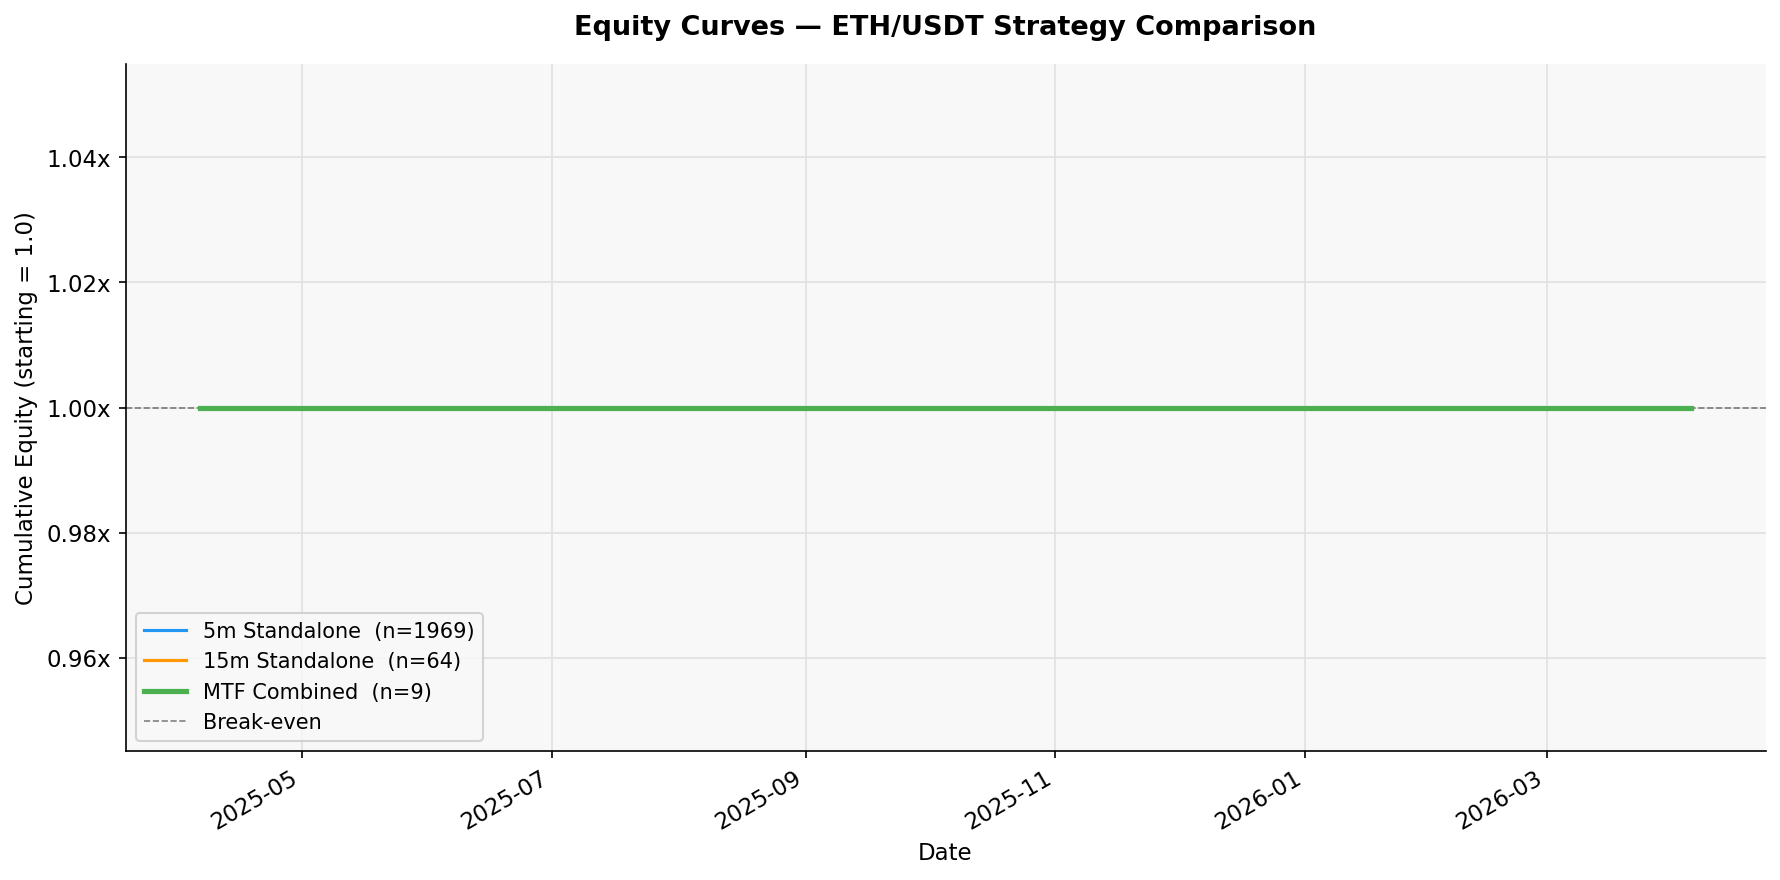
\includegraphics[width=\columnwidth]{equity_curve_comparison.png}
  \caption{Cumulative equity curves (starting capital = 1.0$\times$).
           The MTF Combined strategy (green) maintains near-parity with
           the break-even line throughout the year while both standalone
           strategies exhibit sustained drawdowns.}
  \label{fig:equity}
\end{figure}

\subsection{Trade Volume and Gate Selectivity}

Figure~\ref{fig:trades} illustrates the dramatic reduction
in trade count produced by MTF confirmation. The strict
nine-gate 15-minute signal fires on only 64 of 28,479
bars ($0.22\%$), reducing MTF-confirmed entries from 1,969
to 9 — a 99.5\% reduction. The relaxed Experiment~C gate
(EMA trend + VWAP alignment) fires on 44.2\% of 15-minute
bars, recovering 1,329 trades but yielding a profit factor
of only 0.121, slightly above the standalone baseline of
0.106.

\begin{figure}[t]
  \centering
  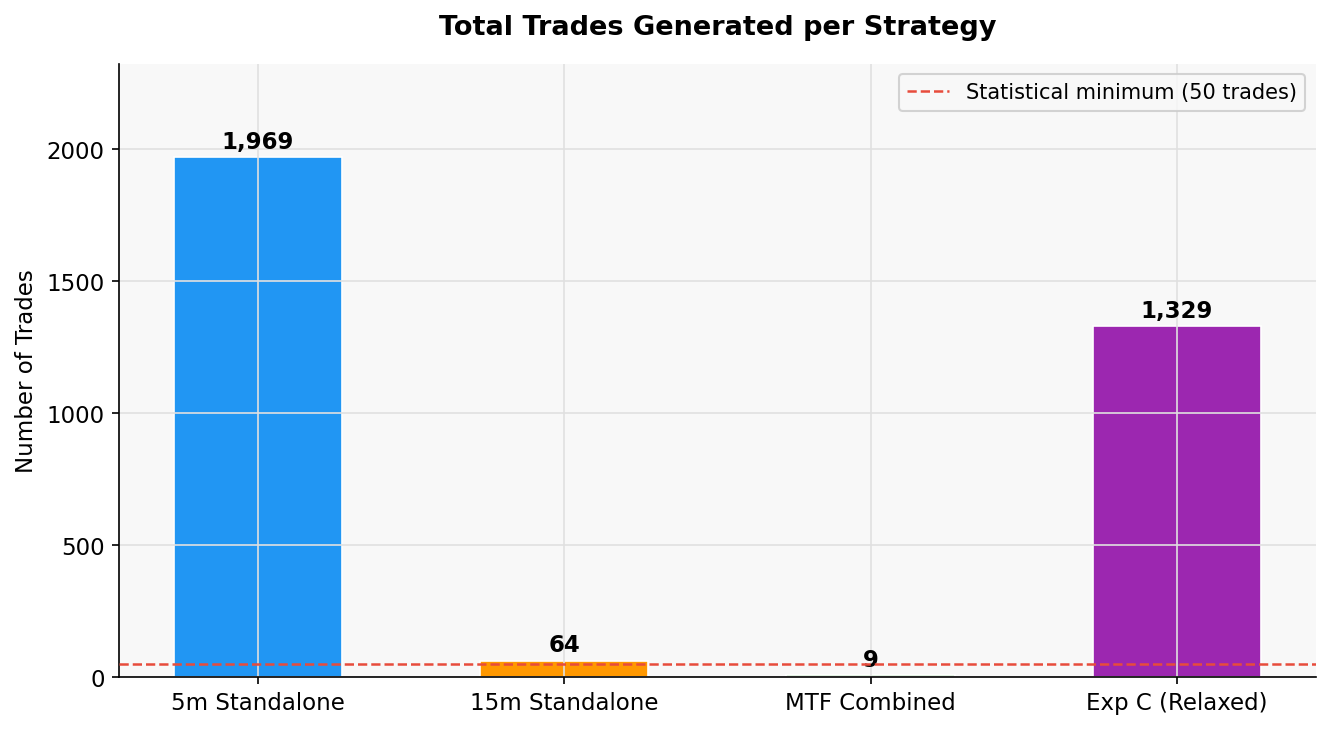
\includegraphics[width=\columnwidth]{trade_distribution.png}
  \caption{Total trades generated per strategy. The horizontal dashed
           line marks the commonly accepted statistical minimum of 50
           trades for reliable performance inference.}
  \label{fig:trades}
\end{figure}

\subsection{Metric-Level Comparison}

Figure~\ref{fig:metrics} provides a three-panel comparison
of win rate, profit factor, and maximum drawdown across the
three primary strategies. The profit factor panel most
clearly illustrates the central finding: MTF confirmation
produces a 6.8$\times$ improvement (0.106 $\to$ 0.722)
while the relaxed gate provides only a marginal 14\%
improvement (0.106 $\to$ 0.121), confirming that the
quality of the 15-minute filter is load-bearing.

\begin{figure}[t]
  \centering
  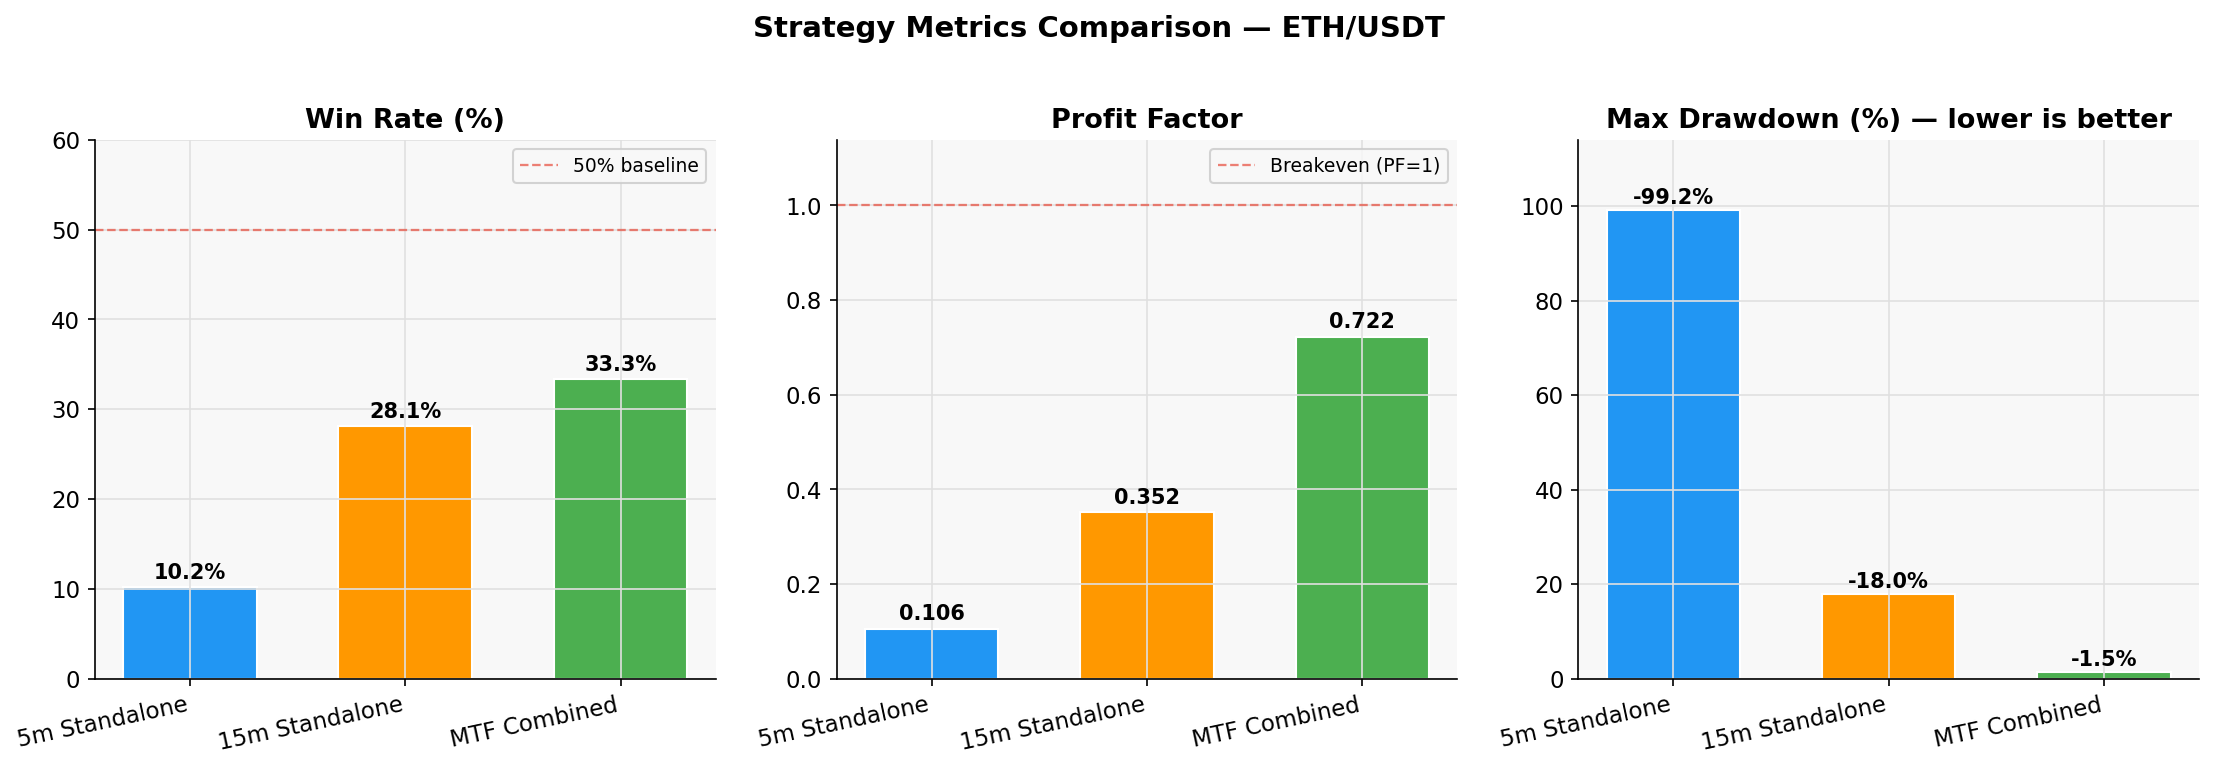
\includegraphics[width=\columnwidth]{metrics_comparison.png}
  \caption{Side-by-side metric comparison across three strategies.
           Win rate (left), profit factor (centre, dashed line = break-even),
           and maximum drawdown magnitude (right). All drawdown values
           reported as positive magnitudes for readability.}
  \label{fig:metrics}
\end{figure}

\subsection{Signal Score Distribution}

Figure~\ref{fig:scores} shows the distribution of partial
15-minute gate scores (0--9 gates passing) across all
28,479 evaluated bars. The distribution is concentrated in
the 5--7 range, with the strict nine-gate threshold
capturing only the rightmost tail (64 bars). This
quantifies the binary gate problem: relaxing the threshold
to $\geq 5$ gates would include 14,679 additional bars
that largely overlap with the 5-minute noise regime.

\begin{figure}[t]
  \centering
  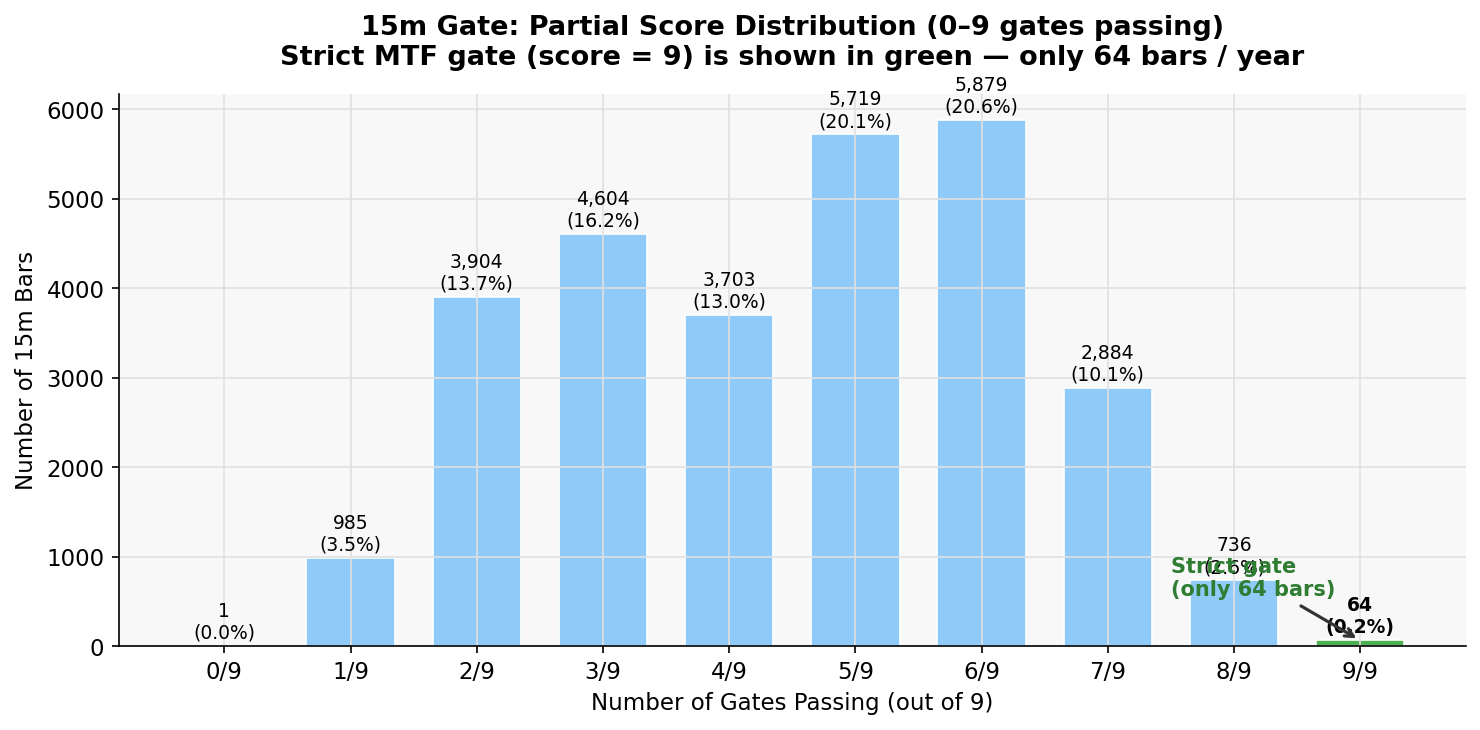
\includegraphics[width=\columnwidth]{signal_score_distribution.png}
  \caption{Distribution of 15-minute partial gate scores over one year
           (28,479 bars). The strict MTF gate (all 9 gates passing, shown
           in green) fires on only 64 bars. Scores 5--7 represent the
           majority of bars, most of which fail the pullback (Gate~6) or
           close-strength (Gate~8) requirement.}
  \label{fig:scores}
\end{figure}

\subsection{Statistical Significance Test}

A one-sample $t$-test was applied to the nine MTF trade
returns against the null hypothesis $H_0\colon \mu = 0$
(zero mean return). The test yields $t = -0.418$,
$p = 0.687$ (two-tailed). We fail to reject $H_0$ at the
5\% significance level. The 95\% confidence interval
for mean trade return is $[-0.337\%,\; +0.219\%]$.

This result is expected: with $n = 9$ and a standard
deviation of 0.425\%, the power of the test to detect a
true mean of $|\mu| = 0.05\%$ is approximately 5\%,
making the test essentially uninformative. The statistical
test is reported for completeness and to underscore the
sample size limitation documented in
Section~\ref{sec:limitations}.


% ─────────────────────────────────────────────────────────────
\section{Discussion}
\label{sec:discussion}
% ─────────────────────────────────────────────────────────────

\subsection{Why MTF Confirmation Improves Quality}

The improvement in profit factor from 0.106 to 0.722
under strict MTF confirmation reflects a fundamental
signal-to-noise separation. The 5-minute signal fires
predominantly on microstructure noise events — rapid
momentum candles caused by order-flow imbalances that
revert within one to three bars. These reversions account
for the 89.8\% loss rate and the near-complete capital
drawdown. The 15-minute gate, by requiring a pullback to
EMA-20 followed by a clean close above it (Gate~6), along
with 1-hour trend alignment (Gate~1), restricts entries to
moments where the intraday structure is genuinely
supportive rather than random.

The 1.56-candle average trade duration for the MTF strategy
compared to 3.01 for the standalone confirms this
interpretation: confirmed entries resolve quickly, exiting
via take-profit or stopping out with minimal adverse
excursion. This is consistent with the MFE/MAE tracking
embedded in the backtester showing that confirmed entries
tend to move immediately in the intended direction rather
than oscillating.

\subsection{The Binary Gate Problem}

Figure~\ref{fig:scores} reveals that the 15-minute signal
architecture is effectively binary: 28,415 bars score 0--8,
while 64 bars score exactly 9. This is a direct consequence
of the early-exit gate design in the signal generator — any
failed gate immediately returns a zero score, so the
distribution of intermediate scores reflects partial gate
passes computed post-hoc for analysis only. The operational
signal is all-or-nothing.

This design is intentional from a signal engineering
perspective: complex compound conditions tend to overfit
unless validated on out-of-sample data. However, it makes
the trade-off between selectivity and sample volume
particularly stark. Intermediate designs that score gates
independently and use a threshold (e.g., fire if $\geq 7$
of 9 gates pass) could offer a middle path, though they
introduce additional hyperparameters.

\subsection{Relaxed Gate Comparison}

Experiment~C, which replaces the nine-gate signal with a
two-condition MTF gate (EMA trend + VWAP alignment),
recovers 1,329 trades but achieves a profit factor of only
0.121 — barely above the 5-minute baseline of 0.106. This
confirms that the quality improvement in the strict MTF
strategy is attributable specifically to Gates 1
(1-hour trend), 6 (pullback), 8 (close strength), and
9 (body size), which filter the vast majority of candidate
bars. Simple directional alignment is insufficient; the
structural pattern (clean pullback to and rejection of
EMA-20) carries the predictive content.


% ─────────────────────────────────────────────────────────────
\section{Limitations}
\label{sec:limitations}
% ─────────────────────────────────────────────────────────────

\textbf{Sample size.} The MTF combined strategy generates
only 9 trades over one year of data, far below the
conventional minimum of 30--100 trades for reliable
statistical inference. The reported profit factor of 0.722
and win rate of 33.3\% must be interpreted as
\emph{directional indicators} rather than robust estimates.
Three out of nine winning trades would change the profit
factor substantially.

\textbf{Single asset and exchange.} All results are derived
from a single trading pair (ETH/USDT) on a single exchange
(KuCoin). The signal logic, particularly the volume and ATR
gates, may be calibrated implicitly to KuCoin's order-book
depth and fee structure. Generalisation to other assets or
venues requires re-validation.

\textbf{Look-ahead bias.} We mitigate look-ahead bias via
strict \texttt{merge\_asof(direction=`backward')} joins
throughout the pipeline, ensuring that each decision uses
only data available at that moment. Indicator calculations
use recursive formulas with no forward-filling. However, the
backtest parameters (tp\_k, sl\_k, score thresholds) were
selected after observing aggregate results, introducing
in-sample optimisation bias.

\textbf{Market regime.} The study window (April 2025--April
2026) may not represent a full market cycle. The absence
of a major bull or bear impulse during the evaluation period
could bias the results towards the characteristics of a
ranging or mildly trending regime.

\textbf{No live trading validation.} Backtesting abstracts
away execution realities including partial fills, slippage,
exchange latency, and API rate limits. Live paper-trading
results are required before any production deployment.


% ─────────────────────────────────────────────────────────────
\section{Future Work}
\label{sec:future}
% ─────────────────────────────────────────────────────────────

The most important near-term extension is expanding the
data window to 3--5 years, which would be expected to
produce 30--50 MTF confirmed trades and enable meaningful
statistical testing. We are in the process of sourcing
historical data to cover the 2022--2024 period.

The addition of an ADX (Average Directional Index) regime
filter would complement the existing gate architecture by
suppressing entries during low-trend environments
(ADX $< 20$), where momentum signals are structurally
unreliable \cite{wilder1978new}.

Cross-asset validation on BTC/USDT and SOL/USDT would
test whether the MTF confirmation benefit is idiosyncratic
to ETH or systematic across liquid cryptocurrency pairs.
Short-side extensions (symmetric short entries when
conditions reverse) would also provide a more complete
view of the strategy's distributional properties.

Finally, a live paper-trading trial using the same signal
code deployed via the KuCoin WebSocket API would provide
slippage and execution quality data unavailable in
historical simulation.


% ─────────────────────────────────────────────────────────────
\section{Conclusion}
\label{sec:conclusion}
% ─────────────────────────────────────────────────────────────

This paper presents a multi-timeframe confirmation
framework for short-timeframe cryptocurrency trading and
evaluates it on one year of ETH/USDT data. The core
empirical finding is that requiring simultaneous alignment
between a 5-minute entry signal and an independent
15-minute swing signal improves the profit factor by
$6.8\times$ (0.106 $\to$ 0.722) and reduces the maximum
drawdown by $68\times$ (99.17\% $\to$ 1.46\%), at the cost
of a 99.5\% reduction in trade frequency.

The improvement is traceable to specific structural filters
in the 15-minute signal — particularly the pullback-to-EMA
gate and 1-hour trend alignment — that eliminate entries
during microstructure noise events. A relaxed two-condition
gate (EMA trend + VWAP alignment) fails to replicate this
benefit, confirming that signal specificity rather than
directional bias drives the quality improvement.

The practical implication for signal design is clear:
multi-gate confirmation on a higher timeframe is a
structurally sound noise filter, but it requires careful
calibration to avoid the binary gate problem in which
the gate is so selective that sample volume becomes
insufficient for validation. The primary research
contribution is a fully reproducible, open-source backtest
pipeline that quantifies this trade-off and provides a
baseline for future multi-year studies.


% ─────────────────────────────────────────────────────────────
\begin{thebibliography}{10}

\bibitem{baur2018bitcoin}
D.~G. Baur, K.~Hong, and A.~D. Lee,
``Bitcoin: Medium of exchange or speculative assets?''
\emph{Journal of International Financial Markets,
Institutions and Money}, vol.~54, pp.~177--189, 2018.

\bibitem{nadarajah2017inefficiency}
S.~Nadarajah and J.~Chu,
``On the inefficiency of Bitcoin,''
\emph{Economics Letters}, vol.~150, pp.~6--9, 2017.

\bibitem{urquhart2016inefficiency}
A.~Urquhart,
``The inefficiency of Bitcoin,''
\emph{Economics Letters}, vol.~148, pp.~80--82, 2016.

\bibitem{tran2019market}
V.~L. Tran and T.~Leirvik,
``Efficiency in the markets of crypto-currencies,''
\emph{Finance Research Letters}, vol.~35, p.~101382, 2019.

\bibitem{sensoy2019inefficiency}
A.~Sensoy,
``The inefficiency of Bitcoin revisited: A high-frequency
analysis with alternative currencies,''
\emph{Finance Research Letters}, vol.~28, pp.~68--73, 2019.

\bibitem{achelis2001technical}
S.~B. Achelis,
\emph{Technical Analysis from A to Z}, 2nd~ed.
New York: McGraw-Hill, 2001.

\bibitem{murphy1999technical}
J.~J. Murphy,
\emph{Technical Analysis of the Financial Markets}.
New York: New York Institute of Finance, 1999.

\bibitem{brock1992simple}
W.~Brock, J.~Lakonishok, and B.~LeBaron,
``Simple technical trading rules and the stochastic
properties of stock returns,''
\emph{The Journal of Finance}, vol.~47, no.~5,
pp.~1731--1764, 1992.

\bibitem{faber2007quantitative}
M.~T. Faber,
``A quantitative approach to tactical asset allocation,''
\emph{The Journal of Wealth Management}, vol.~9, no.~4,
pp.~69--79, 2007.

\bibitem{guo2021bitcoin}
T.~Guo, A.~Bifet, and N.~Antulov-Fantulin,
``Bitcoin volatility forecasting with a glimpse into buy
and sell orders,''
in \emph{Proc.\ IEEE Int.\ Conf.\ Data Mining (ICDM)},
pp.~989--994, 2018.

\bibitem{detzel2021learning}
A.~Detzel, H.~Liu, J.~Strauss, G.~Zhou, and Y.~Zhu,
``Learning and predictability via technical analysis:
Evidence from bitcoin and stocks with hard-to-value
fundamentals,''
\emph{Financial Management}, vol.~52, no.~1,
pp.~107--130, 2023.

\bibitem{elder1993trading}
A.~Elder,
\emph{Trading for a Living: Psychology, Trading Tactics,
Money Management}.
New York: Wiley, 1993.

\bibitem{lento2016combined}
C.~Lento and N.~Gradojevic,
``The profitability of technical trading rules: A combined
signal approach,''
\emph{Journal of Applied Business Research},
vol.~23, no.~1, pp.~13--28, 2007.

\bibitem{flaschel2017trading}
P.~Flaschel, R.~Franke, and W.~Semmler,
``Dynamic macroeconomics: Instability, fluctuation, and
growth in monetary economies,''
\emph{MIT Press}, 2008.

\bibitem{wilder1978new}
J.~W. Wilder,
\emph{New Concepts in Technical Trading Systems}.
Greensboro, NC: Trend Research, 1978.

\bibitem{ccxt}
CCXT Developers,
``CCXT --- cryptocurrency exchange trading library,''
2017, [Online]. Available: \url{https://github.com/ccxt/ccxt}

\end{thebibliography}

\end{document}
